\documentclass{../../myassignment}

\courselabel{IN1080}
\exercisesheet{Assignment 3}{RC filter}
\student{Rolf Vidar Hoksaas}

\usepackage{xfrac}

\newcommand{\ohm}{$\Omega$ }
\newcommand{\volt}{$V$ }
\newcommand{\amperes}{$A$ }
\newcommand{\percent}{$\%$}
\newcommand{\micro}{$\mu$}
\newcommand{\kilo}{$k$}

\begin{document}

	\begin{problem}
		Find $H(j\omega)$ for a low-pass RC filter of the type illustrated in the figure.
	\end{problem}

	\begin{answer}
		Since the impedance $Z_C$ of the condensator equals $\frac{1}{j\omega C}$, can we insert it into the expression:
		\begin{eqnarray*}
			V_{out} &=& \frac{Z_C}{R+Z_C} \cdot V_{in} \\
			V_{out} &=& \frac{1}{\sfrac{R}{Z_C}+1} \cdot V_{in} \\
			V_{out} &=& \frac{1}{R\cdot {j\omega C}+1} \cdot V_{in} \\
		\end{eqnarray*}
		We therefore know the frequency response is $H(j\omega) = \frac{1}{1+j\omega RC}$.
	\end{answer}

	\begin{problem}
		Find the the expression describing the relationship between the amplitude of the input voltage $V_{in}$ and the amplitude of the output voltage $V_{out}$ of the RC filter as a function of frequency.
	\end{problem}

	\begin{answer}
		The relationship between the output value of the voltage and its input is given by
		\begin{eqnarray*}
			V_{out}(t) &=& |H(j\omega)|\cdot V_{in}(\omega, t)\\
			V_{out}(t) &=& |H(j\omega)|\cdot cos(\omega t + \phi_c)\\
			V_{out}(t) &=& \frac{1}{\sqrt{1+(\omega RC)^2}}\cdot cos(\omega t + \angle H(j\omega))\\
			V_{out}(t) &=& \frac{1}{\sqrt{1+(\omega RC)^2}}\cdot cos(\omega t + \arctan(\omega RC))\\
		\end{eqnarray*}
		and we know the boundaries of the cosinus is $\pm 1$, therefore the amplitude is given by
			\begin{eqnarray*}
				A_{out} = |H(j\omega)| = \frac{1}{\sqrt{1+(\omega RC)^2}}
			\end{eqnarray*}

	\end{answer}

	\newpage

	\begin{problem}
		Assume $C=22nF$, and that we want the cutoff frequency of the filter to be 200Hz. Find $R$. The cutoff frequency is defined as the frequency where the amplitude of the output signal is $\sfrac{1}{\sqrt{2}}\approx 0.7071$ times the amplitude of the input signal.
	\end{problem}

	\begin{answer}
		Given
		\begin{eqnarray*}
			H(j\omega) = \frac{1}{\sqrt{1+j\omega RC}}
		\end{eqnarray*}
		and the definition of cutoff frequency (where the cutoff frequency is $\sfrac{1}{\sqrt2}$ the DC voltage, thereby the frequency being $0$.)
		\begin{eqnarray*}
			|H(j\omega_c)| &=& \frac{1}{\sqrt{1+(\omega_c RC)^2}} = \frac{1}{\sqrt2}H(j0) \\
			&\implies& \frac{1}{\sqrt{1+(\omega_c RC)^2}} = \frac{1}{\sqrt2} \\
			&\implies& \sqrt{1+(\omega_c RC)^2} = \sqrt2 \\
			&\implies& 1+(\omega_c RC)^2 = 2 \\
			&\implies& (\omega_c RC)^2 = 1 \\
			&\implies& \omega_c = \frac{1}{RC}
		\end{eqnarray*}

		We can therefore say that the resistance for the desired cutoff frequency is $R = \sfrac{1}{w_c C}$, and since $w_c = \tau \cdot f_c$, it is equivalent to saying 
		\begin{eqnarray*}
			R &=& \frac{1}{\tau \cdot f_c \cdot C} \\
			  &=& \frac{1}{\tau \cdot 200[Hz] \cdot 22[nF]} \\
			  &=& \frac{10^7}{\tau \cdot [Hz] \cdot 44[F]} \\
			  &\approx& 36.2k\Omega
		\end{eqnarray*}
	\end{answer}

	\newpage

	\begin{problem}
		For the value you have found for $R$, and a capacitor value of $C=22nF$, use Matlab and plot the ratio of the amplitude of the input signal to the amplitude of the output signal ($|H(j\omega)|$), for frequencies in the range 0-20kHz.
	\end{problem}

	\begin{problem}
		Do the same for $R= 10k\Omega$ and combine the two curves together in a single plot.
	\end{problem}

	\begin{answer}
		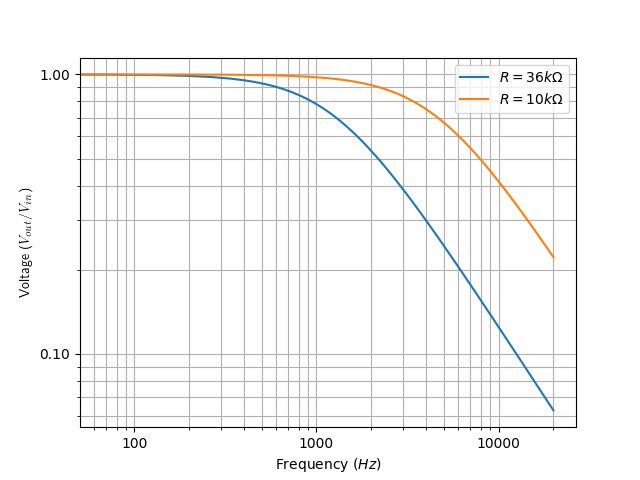
\includegraphics{scalarlowpassfilter.png}
	\end{answer}

	\newpage

	\begin{problem}
		Make an new plot of the curves found in question 4/5 using logarithmic axes by replacing ”plot()” with”loglog()” in Matlab.  Follow with the command ”ylim([0.01 2])” and ”grid on”, to get a better view
	\end{problem}

	\begin{answer}
		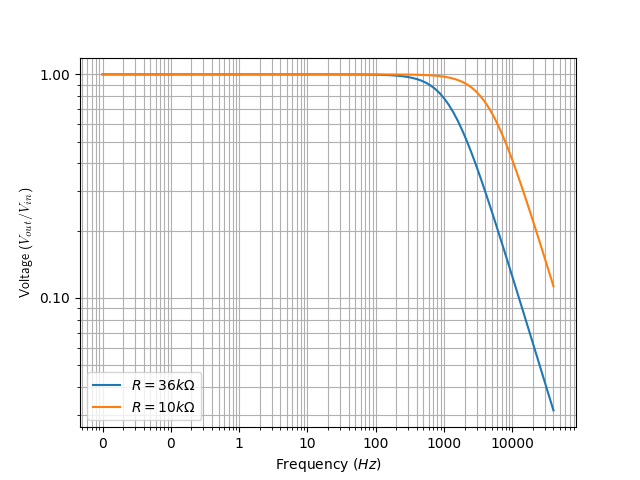
\includegraphics{logarithmiclowpassfilter.png}
	\end{answer}

\end{document}